%%% Local Variables:
%%% mode: latex
%%% TeX-master: "../report"
%%% End:

To describe the overall design of the Kite compiler, we will start by
breaking it down into general parts, where each part or module has a
specific task. Below we have a waterfall model including the main
parts of the compiler:

\begin{figure}[H]
  \label{fig:flow}
  \center
  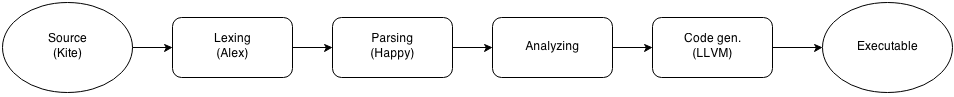
\includegraphics[scale=0.45]{images/flow.png}
  \caption{General flow of the Kite compiler}
\end{figure}

At first it can seem a little daunting, but when we get into the
purpose of each step, there will be a more obvious flow.

\subsection{Preprocessor}
The first thing the compiler does is preprocess the input, e.i. the
source code files, that it has been given. This is quite simply the
task of including all necessary files into one file. The files to be
included are declared in the top of the file.

\begin{figure}[H]
  \label{fig:preprocessor}
  \center
  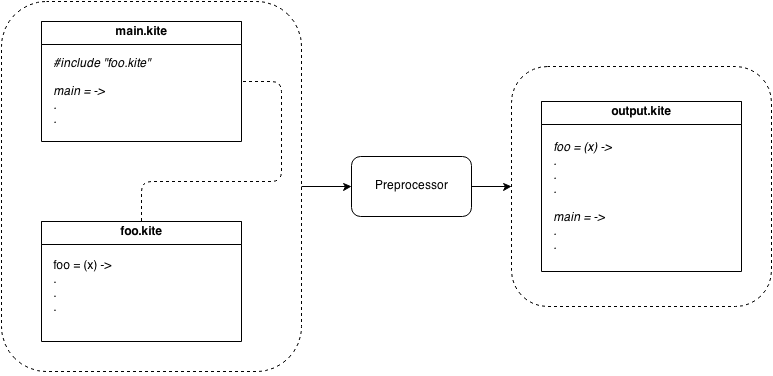
\includegraphics[scale=0.45]{images/preprocessor.png}
  \caption{Input and output of the Preprocessor}
\end{figure}

The nature of the preprocessor is quite simple, as the only task it
simple textual substitution.

\subsection{Lexical analysis}
The lexical analyzer, or just \emph{lexer}, is a central part of most
compilers. It has the important task of processing some input and
converting it to known, referencable tokens. This process is commonly
known as \emph{tokenization}.

Most lexers as quite simple, and does not contain much
complexity. That is often reserved for the parser and analyzer, which
we will come back to next.

\subsection{Parser}
The parser takes the string of tokens from the lexer, and based on a
language grammar, builds a corresponding data structure, namely the
parse tree. In the process it check that that the input is
syntactically correct. Therefor, this process is also called syntactic
analysis.

\subsection{Desugar}

\subsection{Analyzer}

\subsection{Optimizer}

\subsection{Code generation}
